\documentclass[11pt,a4paper]{article}
\usepackage[left=2cm,right=2cm,top=2cm,bottom=3cm]{geometry}
\usepackage{amsmath,amsfonts,amsthm,amssymb,varioref,times}
\usepackage{gensymb}
 \usepackage[explicit]{titlesec}
    % Raised Rule Command:
    % Arg 1 (Optional) - How high to raise the rule
    % Arg 2 - Thickness of the rule
    \newcommand{\raisedrulefill}[2][0ex]{\leaders\hbox{\rule[#1]{0.5pt}{#2}}\hfill}
    \titleformat{\section}{\Large\bfseries}{\thesection. }{0em}{#1\,\raisedrulefill[.5ex]{0.5pt}}

%to resume numbering in a list
\usepackage{enumitem}

%pour ecrire en français avec les accents
\usepackage[utf8]{inputenc}
\usepackage[T1]{fontenc}
\usepackage{lmodern} % load a font with all the characters
\usepackage{units}

%Image-related packages
\usepackage{wrapfig}
\usepackage{float, graphicx}
\graphicspath{ {./img/} }
\usepackage{subcaption}
\usepackage[export]{adjustbox}


%pour faire des cadres
\usepackage{framed}
\usepackage[dvipsnames]{xcolor}
\usepackage{tcolorbox}
\usepackage{tikz}

%chemistry frmulae
\usepackage{chemfig}
\usepackage{chemformula}
 

% parametres des entete et de pieds de pages
\usepackage{fancyhdr}
\pagestyle{fancy}
\fancyhf{}
\lhead{SciPhy : 2nde}
\rhead{Exercices - Réfraction}
\chead{2019-27}
\rfoot{Page \thepage}
\lfoot{SZayyani}


% pour ecrire sur +sieurs colonnes
\usepackage{multicol}
\setlength{\columnseprule}{0.25pt}
\setlength{\columnsep}{60pt}

% Fusion de lignes de tableaux.
\usepackage{multirow}

% Position verticale des lettres dans la ligne de tableau.
\usepackage{array}


% MATH -----------------------------------------------------------
\newcommand{\To}{\longrightarrow}
\newcommand{\gpl}{\; g\cdot L^{-1}}
\newcommand{\gpmol}{\; g\cdot mol^{-1}}
\newcommand{\mpl}{\; mol\cdot L^{-1}}
\newcommand{\mps}{\; m\cdot s^{-1}}
\newcommand{\mpss}{\; m\cdot s^{-2}}
\newcommand{\es}[1]{\cdot10^{#1}}
\newcommand{\eng}[1]{(\textcolor{purple}{= #1})}
\newcommand{\norm}[1]{\left\Vert#1\right\Vert}
\newcommand{\abs}[1]{\left\vert#1\right\vert}

\newenvironment{eg}
 {\begin{shaded} \textbf{Exemple:} } { \end{shaded}}

\newcounter{exo}
\newenvironment{exo}[1][]
 {\refstepcounter{exo} \begin{shaded}\noindent $\triangleright \quad$\textbf{Exercice~\theexo. #1} } { \end{shaded}}    

\newenvironment{defn}[1]
 {\begin{leftbar}\noindent \textbf{Définition :\textit{ \quad #1} } } { \end{leftbar}} 
\newenvironment{rmrq}
 {\begin{shaded} \textbf{Remarque: Pour aller plus loin ...}\\ \itshape } { \end{shaded}}


\definecolor{shadecolor}{gray}{0.8}

\title{Exercices - Réfraction}
\date{}
\author{}

\setlength{\parindent}{0mm}
\setlength{\parskip}{2mm}


\begin{document}
\maketitle
\vspace{-1.9cm}

%%%%%%%%%%%%%%%%%%%%%%%%%%%%%%%%%%%%%%%%%%%%%%
\section{Lumière traversant un prisme droit}

\begingroup
\setlength{\intextsep}{0pt}%
\setlength{\columnsep}{0pt}%
\begin{wrapfigure}{r}{0.55\textwidth}
    \centering
\begin{tikzpicture}[scale=0.5]

% baseline
\draw (1,0) -- (18,0) ; 

%triangle 
\draw[very thick] (5,0) -- (5,10) -- (10,0) -- (5,0); 
\draw (5,0) node [below]{$A$} ; 
\draw (5,10) node [above]{$C$} ; 
\draw (10,0) node [below]{$B$} ; 
\draw (16,0) node [below]{$D$} ; 
\draw (5,4.5) node [right]{$I$} ; 
\draw (8,4.5) node [right]{$J$} ; 
\draw (5,0) rectangle (5.5,0.5) ; 

%rayon lumineux
\draw[dashed, ->] (1,4) -- (2,4) ; 
\draw[dashed, ->] (2,4) -- (5,4) -- (7.9,4) -- (16,0) ;  
\draw [dotted] (1,4) -- (16,4) ; 

%angles 
\draw (4.75,4) rectangle (5,4.25) ; 
%\draw (14.9,0.5) arc (150:180:1cm);
\draw (5,9) arc (270:298:1cm) ; 
\draw (13,4) arc (0:-44:3cm);
\draw (12,3.5) node [below]{\large{$\theta$}} ;
\end{tikzpicture}
\end{wrapfigure}

Considérer le prisme en verre ($n_{verre}=1,52$) dans la figure ci-après. 

Le rayon lumineux arrive, dans l'air, parallèle au sol. En traversant le prisme le rayon sera dévié comme sur la figure, et arrive au niveau du sol au point $D$. 

En sachant que l'angle au sommet $\angle ACB = 30\degree$ déterminer l'angle de déviation $\theta$ du rayon en sortant du prisme.

\endgroup
\vspace{1cm}

%%%%%%%%%%%%%%%%%%%%%%%%%%%%%%%%%%%%%%%%%%%%%%
\section{Lumière traversant un prisme droit - encore}

Nous nous trouvons face à la même situation que dans l'exercice précédent, avec la seule modification que le rayon incident n'est plus parallèle au sol. Le rayon incident arrive maintenant en point $I$ avec un angle d'incidence $i_1 = 30\degree$.
\begin{enumerate}
    \item Déterminer l'angle $\angle BDJ$ que se formera entre le sol et la rayon sortant du prisme.
    \item A partir de quel $i_1$ à l'entrée du prisme le rayon subit-il une réflexion totale interne dans le prisme? 
\end{enumerate}

\begin{center}
    \begin{tikzpicture}[scale=0.7]

% baseline
\draw (1,0) -- (18,0) ; 

%triangle 
\draw[very thick] (5,0) -- (5,10) -- (10,0) -- (5,0); 
\draw (5,0) node [below]{$A$} ; 
\draw (5,10) node [above]{$C$} ; 
\draw (10,0) node [below]{$B$} ; 
\draw (16,0) node [below]{$D$} ; 
\draw (5,4.5) node [right]{$I$} ; 
\draw (8.25,4.5) node [right]{$J$} ; 
\draw (5,0) rectangle (5.5,0.5) ; 

%rayon lumineux
\draw[dashed, ->] (1,2) -- (5,4) ; 
\draw[dashed, ->] (5,4) -- (7.7,4.6) -- (16,0) ;  
\draw [dotted] (1,4) -- (7,4) ; 

%angles 
\draw (4.75,4) rectangle (5,4.25) ; 
\draw (14,1.1) arc (145:180:2cm);
\draw (14.2,1) arc (145:180:1.8cm) ;
\draw (5,9) arc (270:298:1cm) ; 
\draw (3.1,4) arc (180:215:1.4cm) ; 
\draw (2.8,4) node [below]{\large{$i_1$}} ; 
%\draw (13,4) arc (0:-44:3cm);
%\draw (12,3.5) node [below]{\large{$\theta$}} ;
\end{tikzpicture}
\end{center}

\section{Lumière traversant une lame en verre}

\begingroup
\setlength{\intextsep}{0pt}%
\setlength{\columnsep}{0pt}%
\begin{wrapfigure}{r}{0.35\textwidth}
    \centering
    \includegraphics[width=.95\linewidth]{refraction/BeamTranslation.png}
\end{wrapfigure}

Considérer une lame en verre d'épaisseur $e$ comme la figure ci-contre. Un rayon monochromatique arrive sur la première surface en en point que l'on appelle $I$. Le rayon arrive sur cette surface avec un angle d'incidence $i_1$. 

Le rayon va subir une première réfraction en entrant dans la lame de verre, et puis une deuxième réfraction à la sortie. 

\begin{enumerate}
    \item Montrer que le rayon sortant est parallèle au rayon entrant en point $I$. 
    \item Déterminer l'expression littérale du décalage $\Delta y$ des deux rayons, en fonction de l'épaisseur $e$ et l'angle d'incidence $i_1$ en point $I$. 
    \item Calculer la valeur de $\Delta y$. 
\end{enumerate}

\begin{tcolorbox}[title=Données]
$n_{air}=1,00$  \quad ; \quad  $n_{verre}=1,50$  \quad ; \quad $e=3,0\; cm$
\end{tcolorbox}

\endgroup

\section{Lumière traversant un prisme équilatéral}

\begingroup
\setlength{\intextsep}{0pt}%
\setlength{\columnsep}{0pt}%
\begin{wrapfigure}{r}{0.5\textwidth}
    \centering
    \includegraphics[width=.95\linewidth]{refraction/prisme2.jpg}
\end{wrapfigure}

Considérons maintenant un prisme équilatéral en verre. 

Comme pour Ex. 1, Nous avons un rayon lumineux incident sur une des faces du prisme qui est parallèle au sol. 

Déterminer l'angle $i_4$. 

\endgroup
\vspace{1cm}
\begin{tcolorbox}[title=Données]
$n_{air}=1,00$, $n_{verre}=1,50$  
\end{tcolorbox}

\section{Lumière traversant un prisme équilatéral II}
\begingroup
\setlength{\intextsep}{0pt}%
\setlength{\columnsep}{0pt}%
\begin{wrapfigure}{r}{0.55\textwidth}
    \centering

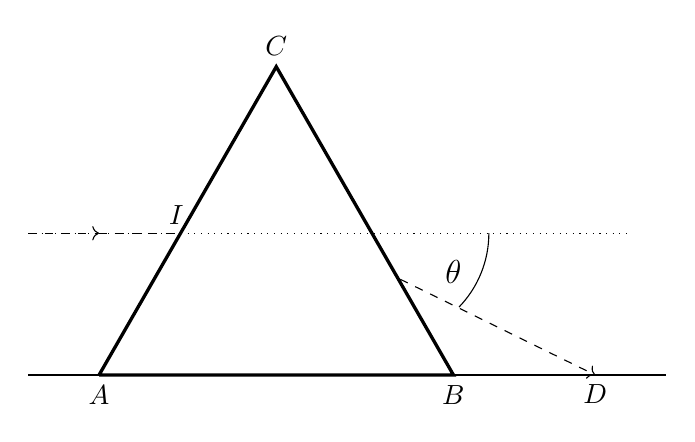
\begin{tikzpicture}[scale=0.45]

% baseline
\draw (0,0) -- (18,0) ; 

%triangle 
\draw[very thick] (2,0) node [below]{$A$} -- (7,8.7) node [above]{$C$} -- (12,0) node [below]{$B$} -- (2,0); 
\draw (16,0) node [below]{$D$} ; 
\draw (3.7,4.5) node [right]{$I$} ; 

%rayon lumineux
\draw[dashed, ->] (0,4) -- (2,4) ; 
\draw[dashed] (2,4) -- (4.3,4) ; 
\draw[dashed, ->] (10.5,2.7) -- (16,0) ;  
\draw[dotted] (0,4) -- (17,4) ; 


%angles 
\draw (13,4) arc (0:-44:3cm);
\draw (12,3.5) node [below]{\large{$\theta$}} ;
\end{tikzpicture}
\end{wrapfigure}

Considérons le même prisme que dans l'exercice précédent. 

Cette fois nous allons comparer un tel prisme d'abord en plexiglas, et puis en diamant.

\begin{enumerate}
    \item Déterminer l'angle $\theta$ de la déviation du rayon lumineux à la sortie du prisme. 
    \item A partir de quel indice de réfraction est-ce que le rayon incident subirait une réflexion totale interne?
    \item $[$BONUS$]$ A partir de quel indice de réfraction (du prisme) le rayon subirait une réflexion totale interne sur la deuxième face du prisme (l'empêchant de sortir). Déterminer son expression littérale mais aussi sa valeur numérique. 
\end{enumerate}

\begin{tcolorbox}[title=Données]
$n_{air}=1,00$ \quad ; \quad $n_{diamant}=2,40$\quad ; \quad $n_{plexiglas}=1,65$\quad ; \quad $\alpha=30\degree$  
\end{tcolorbox}

\endgroup

\section{La fibre optique}
Nous allons maintenant étudier le principe de la fibre optique. On se rappelle que la fibre optique permet la propagation d'un rayon lumineux dans son coeur en raison du fait que l'indice de réfaction de ce dernier $n_1$ est supérieur à celui $n_2$ de la gaine l'entourant (c.f. schéma ci-dessous). 

\begin{figure}[h]
    \centering
    \includegraphics[width=0.9\textwidth]{refraction/fibre1.jpg}
\end{figure}

\begin{enumerate}
    \item Déterminer et calculer l'angle de réfraction en $A$ pour $\alpha = 30\degree$. 
    \item Calculer l'angle d'incidence $i$ du rayon en point $J$ (un peu de géométrie). 
    \item Déterminer et calculer l'angle critique $\theta_J$ à partir duquel le rayon incident en $J$ subirait une réflexion totale interne. 
    \item Déterminer l'angle critique $\theta_A$, à l'entrée de la fibre, à partir duquel le rayon arrivant en $J$ subirait une réflexion totale internet. 
    \item Déterminer l'intervalle de valeur pour l'angle d'entrée $\alpha$ pour lequel le rayon entrant dans la fibre optique se propagerait dans la fibre par réflexions totales internes, le long de la fibre. 
\end{enumerate}

\begin{tcolorbox}[title=Données]
$n_1=1,49$ \quad ; \quad $n_2=1,45$ \quad ; \quad $n_{air}=1,00$ \quad ; \quad $\alpha=30\degree$  
\end{tcolorbox}

\vspace{1cm}

\section{Un prisme isocèle}
\begingroup
\setlength{\intextsep}{0pt}%
\setlength{\columnsep}{0pt}%
\begin{wrapfigure}{r}{0.3\textwidth}
  \centering\includegraphics[width=0.95\linewidth]{refraction/prisme3.jpg}
\end{wrapfigure}

Le prisme qui nous intéresse est, cette fois, isocèle avec en $AB = BC$.

Le rayon entre perpendiculaire à la face $BC$ au point $I$, et sort de la face $AC$, \textbf{parallèle au rayon incident initial}. 

\begin{enumerate}
    \item Construire la marche du rayon à travers ce prisme depuis le point $I$ au point $K$. Il se peut qu'une réflexion interne totale a lieu à un moment donné. Montrer clairement votre raisonnement.
    \item Déterminer l'indice de réfraction nécessaire pour que le rayon se comporte de cette manière dans le prisme. 
\end{enumerate}

\begin{tcolorbox}[title=Données]
$n_1=1,49$ \quad ; \quad $n_2=1,45$ \quad ; \quad $n_{air}=1,00$ \quad ; \quad $\angle BAC = 40\degree$  
\end{tcolorbox}

\endgroup

\end{document}